\chapter{Work Progress}
\label{chap:work}
\setlength{\parskip}{1.5mm}
%\setlength{\baselineskip}{1.4mm}
\section{Verifying the Algorithm in MATLAB}
\subsection{Model of Non-Linear Dynamic System}
A schematic diagram of the compound triple-pendulum system is shown in Figure 5.1.The bars of the pendulum have significant mass so that it can be modeled as a compound pendulum. The model has been parameterized according to the physical characteristics of the system including mass of the bars, their inertia etc. 
% Damping factors were also included in the model for higher degree of chaos and non-linearity in the system. 
% Each bar ${i}$ is defined by a set of four parameters: 
% ${I_{i}}$, the moment of inertia of the bar, ${m_{i}}$, the mass of the bar,
%  ${L_{i}}$, the length of the bar, and
%  ${k_{i}}$, the damping coefficient of the bar rotating about it’s upper joint. 
The position and velocity of the bars are defined by the six system state variables: $\theta$\textsubscript{1}, $\theta$\textsubscript{2}, $\theta$\textsubscript{3}, ${\dot{\theta\textsubscript{1}}}$, ${\dot{\theta\textsubscript{2}}}$, ${\dot{\theta\textsubscript{3}}}$

%\begin{figure}
%\centering
%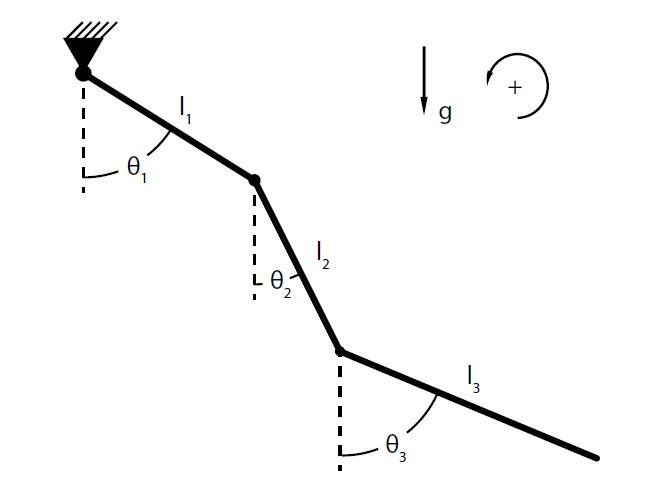
\includegraphics[width=8cm]{pendulum.jpg}
%\caption{Schematic Diagram of Triple Pendulum System}\label{fig:pendulum}
%\end{figure}
% 

\begin{figure}[H]
\begin{subfigure}{0.5\textwidth}
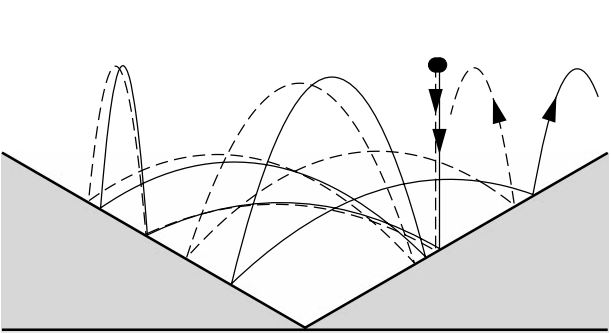
\includegraphics[width=1.1\linewidth]{ball.jpg}
\caption{Chaotic motion of a bouncing ball}\label{fig:ball}
\end{subfigure}
\begin{subfigure}{0.5\textwidth}
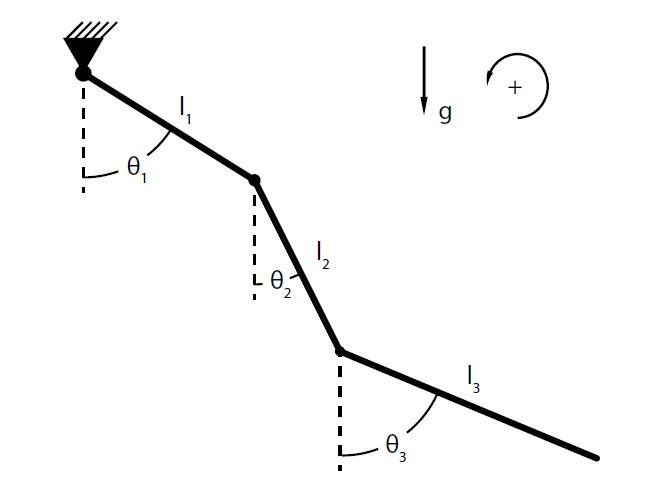
\includegraphics[width=0.8\linewidth]{pendulum.jpg}
\caption{Schematic Diagram of Triple Pendulum}\label{fig:pendulum}
\end{subfigure}
\caption{Examples of Non-Linear Dynamic systems}\label{fig:image1}

\end{figure}
\begin{figure}[h]
\begin{subfigure}{0.5\textwidth}
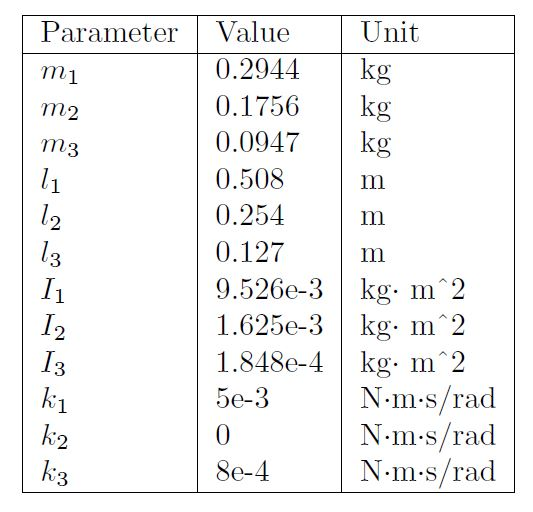
\includegraphics[width=0.8\linewidth]{param.jpg}
\caption{Table 1}\label{fig:param}
\end{subfigure}
\begin{subfigure}{0.5\textwidth}
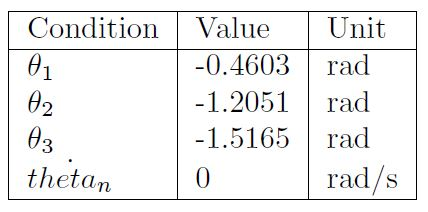
\includegraphics[width=0.8\linewidth]{ic.jpg}
\caption{Table 2}\label{fig:ic}
\end{subfigure}
\caption{Parameters \& Initial Conditions for the Initial Value Problem}\label{fig:image2}
\end{figure}

% \begin{figure}
% 
% 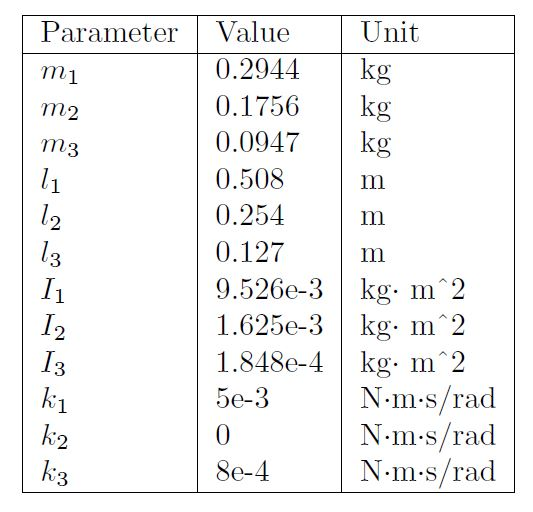
\includegraphics[width=8cm]{param.jpg}
% \caption{Parametric Values used for Simulation}\label{fig:param}
% \end{figure}
% 
% \begin{figure}
% % \centering
% 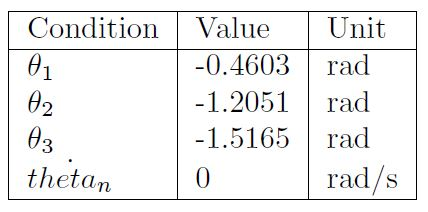
\includegraphics[width=8cm]{ic.jpg}
% \caption{Initial Conditions used for Simulation}\label{fig:ic}
% \end{figure}

\subsection{Simulation of Compound Triple Pendulum}
This compound triple-pendulum model has been simulated using MATLAB using approximate differential equations describing the random motions. The parameters and initial conditions of the ODEs are given in Table 1 and Table 2 respectively. For the simulation, simple numerical methods were used to solve the differential equations and the values corresponding to the angular position of the bars were obtained within a certain duration of time with a predefined precision. This generates the mapping values for the encryption module. 

% \begin{figure}[H]
% \centering
% 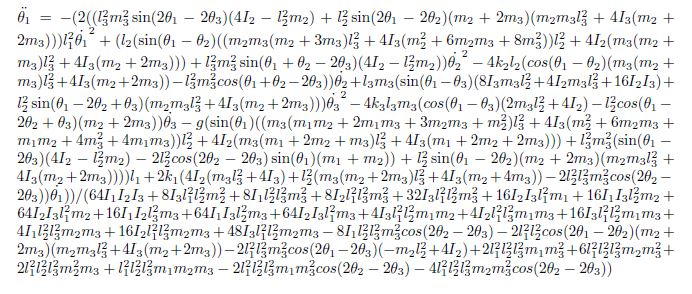
\includegraphics[width=16cm]{diff1.jpg}
% \caption{Differential Equation for ${\theta\textsubscript{1}}$}\label{fig:diff1}
% \end{figure}
% 
% 
% \begin{figure}[H]
% \centering
% 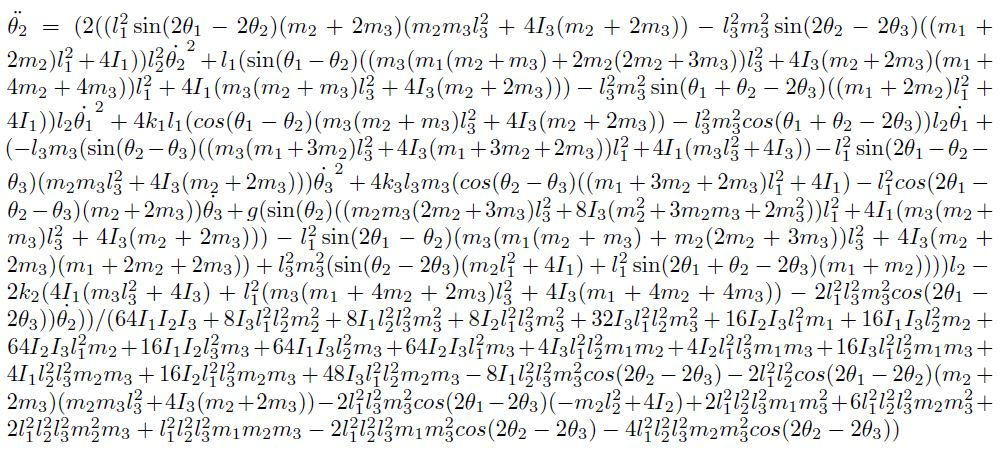
\includegraphics[width=16.5cm]{diff2.jpg}
% \caption{Differential Equation for ${\theta\textsubscript{2}}$}\label{fig:diff2}
% \end{figure}
% 
% 
% \begin{figure}[H]
% \centering
% 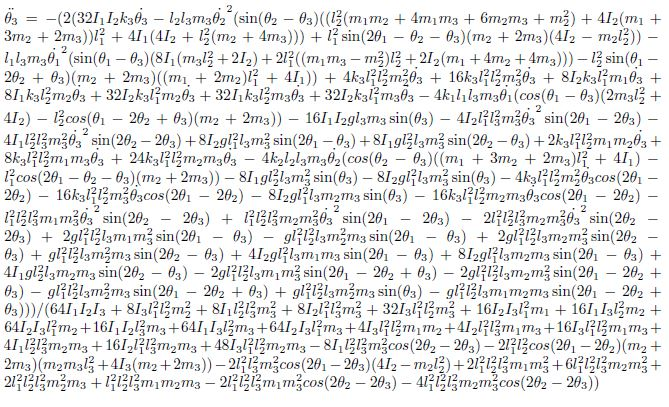
\includegraphics[width=16.5cm]{diff3.jpg}
% \caption{Differential Equation for ${\theta\textsubscript{3}}$}\label{fig:diff3}
% \end{figure}
% \vfill
\subsubsection{Simulation Results}
These are some of the observations from the simulation of the triple-pendulum model for a duration of t = 0 to t = 10 seconds with $\Delta$t = 0.001 :\\
(i) Initial conditions are same as given in Table 1 \& 2:\\
 
\begin{figure}[H]
\begin{subfigure}{0.5\textwidth}
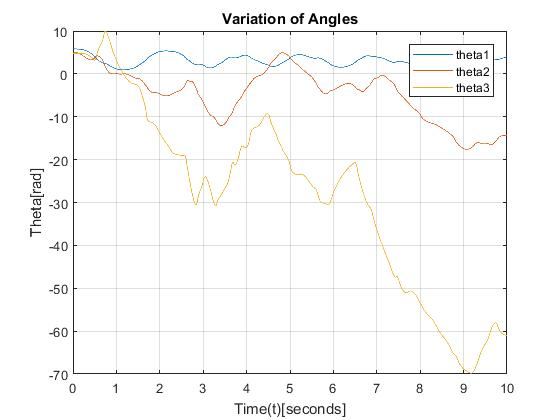
\includegraphics[width=1\linewidth]{theta.jpg}
\caption{Plot of ${\theta}$ vs Time}\label{fig:theta}
\end{subfigure}
\begin{subfigure}{0.5\textwidth}
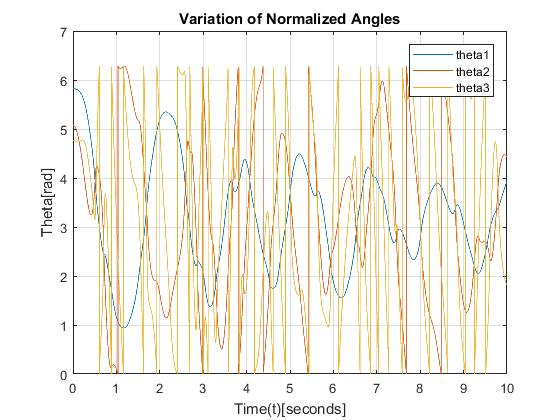
\includegraphics[width=1\linewidth]{theta_norm.jpg}
\caption{Plot of Normalized ${\theta}$ vs Time}\label{fig:theta_norm}
\end{subfigure}
\caption{Motion of Triple-Pendulum for t = 0 to t = 10 sec}\label{fig:image3}
\end{figure}

\begin{figure}[H]
\centering
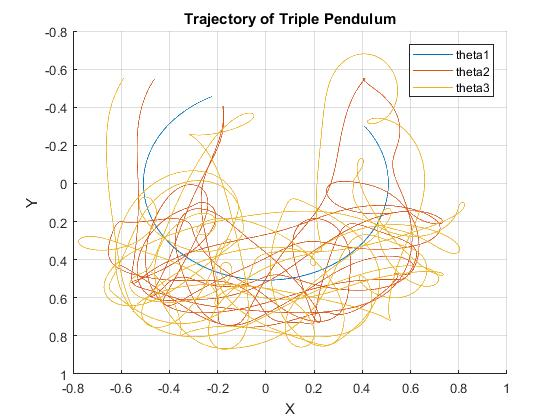
\includegraphics[width=0.7\linewidth]{trajectory.jpg}
\caption{Plot of Motion of Triple-Pendulum}\label{fig:trajectory}
\end{figure}


\subsection{Encryption - Decryption}
Our approach is to convert the plain-text into ascii format and  map the value to the partitioned intervals of the triple-pendulum motion simulated within a specific duration of time for a particular set of parameters and initial conditions. The initial conditions and parameters of the different equation forms a part of the private key. Following the Baptista-type method, the entire range of the chaotic function was partitioned into a number of intervals equal to the number of characters. Each character in the plain-text is then mapped to a specific interval and then to a time point randomly selecting from that interval.  

\begin{figure}[H]
\centering
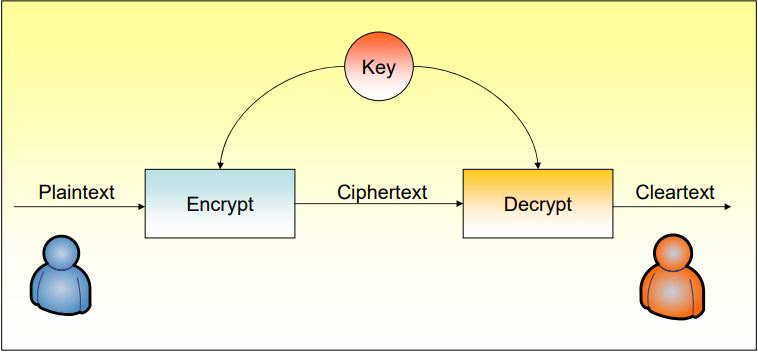
\includegraphics[width=10cm]{crypto.jpg}
\caption{Working Principle of a Symmetric Cryptosystem}\label{fig:crypto}
\end{figure}

On the decryption module, the interval in which the encrypted value lies is computed from the generated motion of the triple-pendulum for the same key and the corresponding index would then refer to the ascii converted clear-text. Converting them into characters, the message can be decoded.\\
\begin{figure}[H]
\centering
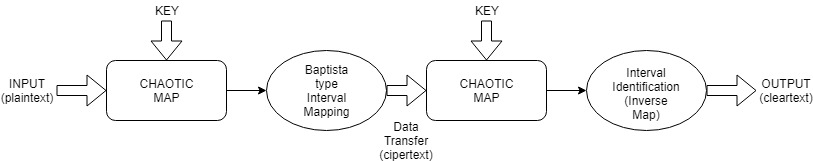
\includegraphics[width=16cm]{Dataflow.jpg}
\caption{Encryption-Decryption Strategy}\label{fig:Dataflow}
\end{figure}


\section{Key Generation}
It is observed that for certain specific parameters or initial conditions, the motion of the bars of the triple-pendulum shows periodic nature after a certain span of time. Hence there is a need to eliminate those parameters or initial conditions for which the motion is periodic as the periodic nature breaks the chaotic behavior of the system. For that a test for periodicity was employed to extract the prominent period of the signal using statistical analysis on the spectrum of the signal. The test used is known as {\bf{\em Fisher's g-statistic test}}(see [11]). This method is based on the test of significance of the periodic components of the signal derived from its periodogram. 

\begin{figure}[H]
\centering
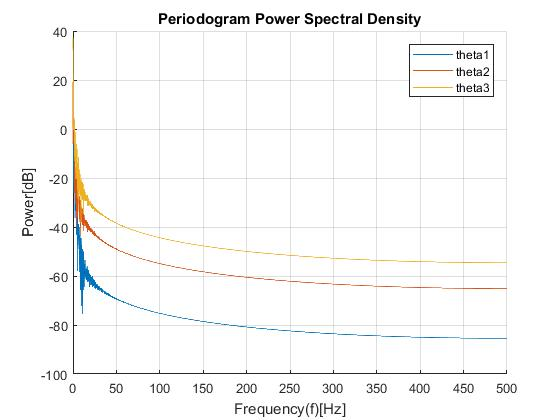
\includegraphics[width=0.7\linewidth]{periodogram.jpg}
\caption{Periodogram Plot for ${\theta}$}\label{fig:periodogram}
\end{figure}


\begin{figure}[H]
\begin{subfigure}{0.5\textwidth}
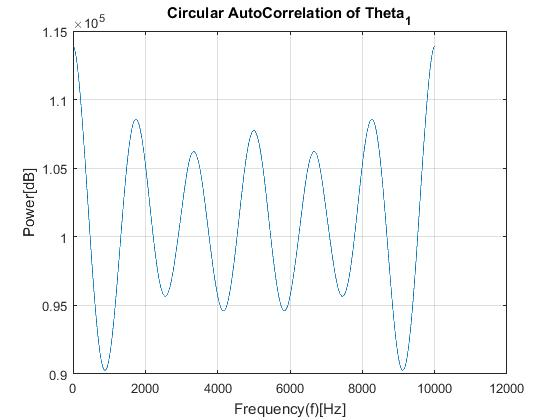
\includegraphics[width=1\linewidth]{auto_corr1.jpg}
\caption{Plot of Circular Auto-Correlation for ${\theta_{1}}$}\label{fig:cir_auto1}
\end{subfigure}
\begin{subfigure}{0.5\textwidth}
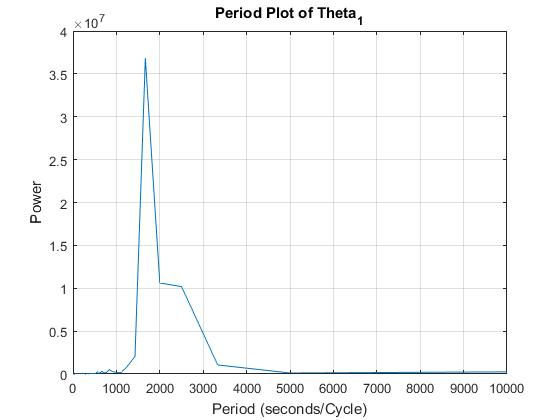
\includegraphics[width=1\linewidth]{period1.jpg}
\caption{Plot of Periodicity for ${\theta_{1}}$}\label{fig:period1}
\end{subfigure}
\caption{Periodic Properties of ${\theta_{1}}$}\label{fig:image4}
\end{figure}

\begin{figure}[H]
\begin{subfigure}{0.5\textwidth}
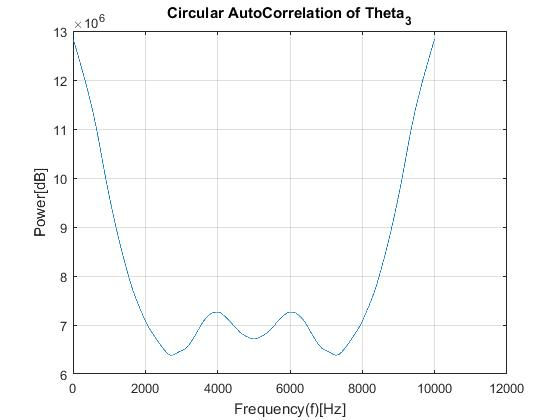
\includegraphics[width=1\linewidth]{auto_corr3.jpg}
\caption{Plot of Circular Auto-Correlation for ${\theta_{3}}$}\label{fig:cir_auto3}
\end{subfigure}
\begin{subfigure}{0.5\textwidth}
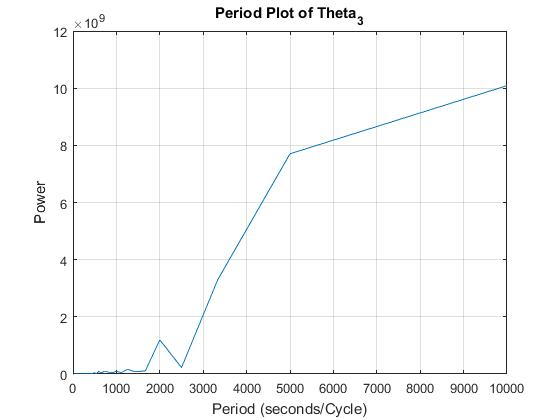
\includegraphics[width=1\linewidth]{period3.jpg}
\caption{Plot of Periodicity for ${\theta_{3}}$}\label{fig:period3}
\end{subfigure}
\caption{Periodic Properties of ${\theta_{3}}$}\label{fig:image5}
\end{figure}

From the figures 5.8 \& 5.9 , it is observed that there is peak at 1700 (seconds/Cycle) for $\theta_{1}$ whereas no such peak occurs for $\theta_{3}$. Thus $\theta_{1}$ is periodic in nature. The values obtained from the periodicity test and plots of circular auto-correlation clearly differentiates the parameters and initial values which leads to periodic nature of the motion and those which lead to non-periodic nature of the motion. Thus by iterating through all possibles values of the parameters and checking likewise for non-periodic nature, a set of keys was generated and stored. 


\section{FPGA Implementation}
The complete design is being implemented at Register-Transfer Level (RTL) in {\bf Verilog HDL} and the target device chosen is Digilent Nexys Board with {\bf Xilinx Artix-7 FPGA}. The following diagram shows the implementation plan for the design :
\begin{figure}[H]
\centering
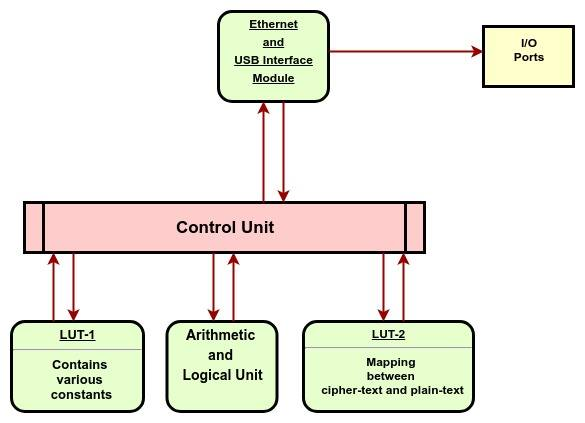
\includegraphics[width=10cm]{fpga_block.jpg}
\caption{Block Diagram of FPGA Implementation}\label{fig:fpga_block}
\end{figure}

1. {\bf Arithmetic and Logical Unit (ALU)} - The ALU uses floating-point arithmetic whose precision can be configured at the time of synthesis. This has been done to enable the study of how security strength varies with arithmetic precision.

2. {\bf Look-Up Table (LUT)} - A fast Look-Up table is to be implemented for storing various constants and the mapping between clear-text and cipher-text.

3. {\bf Ethernet and USB Module} - These are required to enable the device to encrypt or decrypt both a stream of data as well as complete file.

4. {\bf Control Unit} - Essentially a state machine that co-ordinates the operation of all other modules including evaluation of state-variables and transfer of data through USB/Ethernet port.

\section{Analysis}
\subsection{Test for Chaos}
\subsubsection{Collison Test}
\subsection{Test for Randomness}
\subsection{Complexity}
